\footnotetext{Notes from Classical Mechanics by John R. Taylor, ch. 6}

\section{Two example problems}
The calculus of variations can be used to find a function $y(x)$ that minimizes a scalar quantity that is
expressed as an integral $\int_{x_0}^{x_1} f[y(x), y'(x), x] \dx$. \footnote{Note that in physics, the
  independent variable is typically time, and $f$ is a ``Lagrangian'', so the integral is likely to look
  like $\int_{t_0}^{t_1} \Lag(x(t), \xdot(t), t) \dt$.}

Here are two such problems:

\begin{question*}
  What is the shortest path between two points in a plane?
\end{question*}

\begin{proof}
  Let the points be $(x_0, y_0)$ and $(x_1, y_1)$ and let them be joined by some path $y(x)$ of
  length $S$. Consider a short section of the path of length $\Delta s$ above a section of the $x$-axis of
  length $\Delta x$, and make a linear approximation to the path in this region. The length of the hypotenuse
  is
  \begin{align*}
    \Delta s = \sqrt{(\Delta x)^2 + (y'(x)\Delta x)^2} = \sqrt{1 + y'(x)^2} \Delta x.
  \end{align*}

  Therefore a shortest path is a function $y(x)$ that minimizes
  \begin{align*}
    S[y](x_0, x_1) = \int_{x_0}^{x_1} \sqrt{1 + y'(x)^2}\dx.
  \end{align*}
  with the constraint that the endpoints are fixed at $y(x_0) = y_0$ and $y(x_1) = y_1$.

  \todo{Find the function $y$ that minimizes this integral.}
\end{proof}


Can we rephrase  this as a Lagrangian  dependent on position only,  i.e. not involve the  derivative? Let's say
that   there  is   a  scalar   field  $f$   of  constant   value   $f(x,  y)   =  c$.   So  our   task  is   to
minimise $S[y] = \int_{y} c$ where this notation refers to  a path integral along the curve $y(x)$. On the face
of it this is dependent on position only. However, the calculation ends up involving the derivative:
\begin{align*}
  \int_{y} c
  &= c\int_{y}1 \\
  &= c\int_{x_{0}}^{x_{1}}\sqrt{(\dx)^{2} + (y'(x)\dx)^{2}} \\
  &= x\int_{x_0}^{x_1} \sqrt{1 + y'(x)} \dx.
\end{align*}

\begin{question*}
  In 1662 Fermat proposed that light, when passing from one point to another through a material with varying
  refractive index, takes the path which takes least time\footnote{\todo{In fact, the path taken is a
      stationary point with respect to the action? time? ...not necessarily least}}. What is this path?
\end{question*}

\begin{proof}
  Again consider a short section of the path of length $\Delta s$ above a section of the $x$-axis of
  length $\Delta x$. Let $c$ be the speed of light and $n$ be the refractive index in this region. This means
  that the light travels at speed $c/n$, and therefore takes time $(n/c)\Delta s$ to pass along the
  hypotenuse. The refractive index $n$ can vary with both $x$ and $y$, therefore a least-time path is a
  function $y(x)$ that minimizes
  \begin{align*}
    T = \int_{x_0}^{x_1} n(x, y(x)) \d s = \int_{x_0}^{x_1} n(x, y(x)) \sqrt{1 + y'(x)^2} \dx,
  \end{align*}
  with the constraint that the endpoints are fixed at $y(x_0) = y_0$ and $y(x_1) = y_1$.

  \todo{Find the function $y$ that minimizes this integral.}
\end{proof}

A naive thought would be to somehow treat $y$ similarly to how a variable is treated when minimizing a function
in in basic calculus, i.e. differentiate the expression with respect to $y$. Recall that the definition of
derivative is
\begin{align*}
  f'(y_0) = \lim_{y_1 \to y_0}\frac{f(y_1) - f(y_0)}{||y_1 - y_0||}.
\end{align*}

\todo{I think this is nonsense and the reason is that multiplication (and therefore division) of functions is
  not defined (they can be treated as vectors, so can be added and scaled, but do not have an obviously
  appropriate multiplication operation). I don't think choosing a norm would necessarily be problematic.}

\section{The Euler-Lagrange equations}

\begin{proof}
  Note that in both example problems, the integral to be minimized can be viewed as a scalar-valued \emph{functional}
  $S$ that depends on the \emph{function} $y$:
  \begin{align*}
    S[y](x_0, x_1) = \int_{x_0}^{x_1} f[x, y(x), y'(x)] \dx.
  \end{align*}
  The arguments of the function $f$ that is integrated are \emph{not functions}! They are numeric values at a single point
  in the path: the current $x$ value, the current $y$ value, and current slope. We will attempt to stick to a
  notation wherein a symbol like $y$ is a function, and $y(x)$ is a result of evaluating the function at input
  value $x$.

  We'll refer to $S$ as giving the \emph{cost} of traveling along the path $y$, from $(x_0, y_0)$ to $(x_1, y_1)$.

  Recall that we seek a least-cost path $y$, subject to the requirement that the endpoints are $y(x_0) = y_0$
  and $y(x_1) = y_1$. Let $y$ be the least-cost path, and consider an alternative path $Y$ whose cost is
  greater than that of $y$. We can write $Y$ as
  \begin{align*}
    Y = y + \eta,
  \end{align*}
  where we are performing addition on domain-compatible functions\footnote{$(f + g)(x) := f(x) + g(x)$}. The
  difference function $\eta$ must satisfy $\eta(x_0) = \eta(x_1) = 0$ in order to restrict the space of
  functions to those with the same endpoints as $y$. Now introduce a parameter $\alpha \in \R$ and redefine $Y$
  as\footnote{We are adding functions, and we are multiplying a function by a real scalar $\alpha$. The
    resulting function evaluates as $Y(x) = y(x) + \alpha\eta(x).$}
  \begin{align*}
    Y = y + \alpha\eta.
  \end{align*}

  So now we have a family of paths, parameterized by $\alpha$, all satisfying the endpoint requirement, and
  with the least-cost path corresponding to $\alpha=0$. We can reinterpret the cost $S$ so that it is a
  function of $\alpha$:
  \begin{align*}
    S[y](\alpha) &= \int_{x_0}^{x_1} f(x, Y(x), Y'(x)) \dx \\
            &= \int_{x_0}^{x_1} f\(x, y(x) + \alpha\eta(x), y'(x) + \alpha\eta'(x)\) \dx.
  \end{align*}
  We are trying to find a path $y$ that is a minimum in the cost surface over the function space (or a maximum,
  or saddle point). For such a $y$ it must be the case that
  \begin{align*}
    \del_\alpha S[y]\Big|_{\alpha=0} = 0.
  \end{align*}

  So, let's compute $\del_\alpha S[y]$ and use the fact that it must evaluate to zero at $\alpha=0$ to obtain
  an equation that $y$ must obey. We'll assume that $f$ satisfies the (mild) conditions necessary to
  ``differentiate under the integral sign'', i.e. that
  \begin{align*}
    \del_\alpha S = \del_\alpha \int_{x_0}^{x_1} f(x, Y(x), Y'(x)) \dx
                 = \int_{x_0}^{x_1} (\del_\alpha f)(x, Y(x), Y'(x)) \dx.
  \end{align*}

  We have
  \begin{align*}
    Y  &= y + \alpha\eta \\
    Y' &= y' + \alpha\eta',
  \end{align*}
  and so from the chain rule we have
  \begin{align*}
    \del_\alpha f &= \del_{Y(x)} f \cdot \del_\alpha Y + \del_{Y'} f \cdot \del_\alpha Y' \\
                 &= \del_{Y} f \cdot \del_\alpha Y + \del_{Y'} f \cdot \del_\alpha Y' \\
  \end{align*}

  \begin{align*}
    \pdv{f(Y, Y', x)}{\alpha} &= \pdv{f}{Y}\pdv{Y}{\alpha} + \pdv{f}{Y'}\pdv{Y'}{\alpha} \\
                              &= \pdv{f}{Y}\eta + \pdv{f}{Y'}\eta'.
  \end{align*}
  Plugging this into the expression for $\pdv*{S}{\alpha}$ and evaluating at $\alpha = 0$ we have
  \begin{align*}
    \int_{x_0}^{x_1} \(\eta\pdv{f}{y} + \eta'\pdv{f}{y'}\) \d x = 0.
  \end{align*}
  (I believe that $Y$ and $Y'$ have now become $y$ and $y'$ because we are evaluating at
  $\alpha=0$.)

  Now, recall integration by parts, $\int_a^b u \dv{v}{x} \d x = [uv]_a^b - \int_a^b v\dv{u}{x}\d x$, and apply
  it to the second term inside the integral:
  \begin{align*}
    \int_{x_0}^{x_1} \eta'\pdv{f}{y'} \d x = \Bigg[\eta\pdv{f}{y'}\Bigg]_{x_0}^{x_1} - \int_{x_0}^{x_1} \eta\(\dv{}{x}\pdv{f}{y'}\)\d x.
  \end{align*}
  Because $\eta$ was defined to be the difference between two candidate paths, as noted above we have
  that $\eta(x_0) = \eta(x_1) = 0$. Thus the first term (the ``endpoint term'' or ``boundary term'') is
  zero\footnote{According to Taylor this is common in physics, i.e. that the endpoint term is zero and thus
    integration by parts results in ``switching the prime'' from one factor to the other under the integral, and
    applying a negation.}. So now we have
  \begin{align*}
    \int_{x_0}^{x_1} \eta(x)\(\pdv{f}{y} - \dv{}{x}\pdv{f}{y'}\) \d x = 0.
  \end{align*}
  We now argue that this means that the difference-of-derivatives-function inside the integral is zero for
  all $x$. The reason is basically that this equality is true for \emph{any} $\eta(x)$. So suppose the
  difference-of-derivatives-function were not equal to zero for some $x$. Then we could construct an $\eta(x)$
  that is non-zero for the same $x$ values that the difference-of-derivatives-function is non-zero for, the
  upshot being that we could construct things so that the value of the integral is non-zero; a
  contradiction. Therefore the difference-of-derivatives-function is zero for all $x$, and we have the
  Euler-Lagrange equations:
  \begin{align*}
    \pdv{f}{y} - \dv{}{x}\pdv{f}{y'} = 0.
  \end{align*}
\end{proof}

This is a system of differential equations which must be satisfied by any path that is stationary with respect
to $f$.

In SICM's functional notation, the Euler-Lagrange system of equations is
\begin{align*}
    (\del_1 f \circ \Gamma[q]) - D(\del_2f \circ \Gamma[q]) = 0,
\end{align*}
where
\begin{itemize}
\item $\Gamma$ is a function mapping time to the tuple of arguments taken by $f$, i.e. $\Gamma[q](t) = (t, y(t), y'(t))$,
\item $\del_1$ refers to the partial derivative with respect to position and $\del_2$ is with respect to velocity
  (zero-based indexing of positional arguments).
\end{itemize}

So, any path $q$ for which the action is stationary satisfies the Euler-Lagrange system of differential
equations. And what those equations say is the following:
\begin{enumerate}
\item Recall that $f$ is a function of time, position and velocity values at a single moment in time.

\item Compute the partial derivative function of $f$ with respect to the position argument. Note that this is a
  function of time, position and velocity; its output is a real number (the slope of a certain tangent line to
  the real-valued $f$ surface).

\item Now, form a new function by composing this partial derivative function with $\Gamma[q]$. The new function
  maps time to a real number (the slope). Call this function $A$.

\item Repeat the previous two steps for the velocity argument, instead of the position argument. So again, the
  result is a function mapping time to a real number. But this time, take the time derivative of that
  function. The result is still a function mapping time to a real number. Call this function $B$.

\item Now, take a candidate path $q$. If the action is stationary along that path, then at every moment $t$ we will
  find that $A(t) = B(t)$.
\end{enumerate}

\section{Examples}

\subsection{The shortest path between two points on a plane}

\subsubsection{Functional notation}

\begin{question*}

\end{question*}

Let's return to this problem, using the functional notation. We have
\begin{proof}
  \begin{itemize}
  \item $f(x, y, v) = (1 + v^2)^{1/2}$ \\
    A function mapping the local tuple to the cost associated with that point in the path.

  \item $(\del_1 f)(x, y, v) = 0$ \\
    Partial derivative of $f$ with respect to its second argument.

  \item $(\del_2 f)(x, y, v) = v(1 + v^2)^{-1/2}$ \\
    Partial derivative of $f$ with respect to its third argument.

  \item $q(t) = y(t)$ \\
    The path: a map from time to spatial coordinate.

  \item $(\del_2 f \circ \Gamma[q])(t) = y'(t)(1 + y'(t)^2)^{-1/2}$ \\
    Composing $\del_2 f$ with $\Gamma[q]$ represents ``plugging in'' $y'(t)$ as the value of $v$.

  \item Recall the Euler-Lagrange equation, which is true for any $q$ for which the action is minimized:
    \begin{align*}
    D(\partial_2f \circ \Gamma[q]) - \partial_1f \circ \Gamma[q] = 0.
    \end{align*}

  \item Since the partial derivative $\partial_1f$ with respect to the position argument is zero, the
    Euler-Lagrange equation states that for the action to be minimized we must have
    \begin{align*}
     D (\del_2 f \circ \Gamma[q])(t)
     = \(\frac{y'}{(1 + y'^2)^{1/2}}\)'
     = 0.
    \end{align*}

  \item In other words, $\frac{y'}{(1 + y'^2)^{1/2}}$ is constant, which leads to
    $y' = \sqrt{C/(1 - C)}$, where $C$ is a constant.

  \item So $y'$ is constant, i.e. a straight line.
  \end{itemize}
\end{proof}

\subsubsection{Traditional notation}
\begin{proof}
  Let $\r = (x, y)$. We want to find the $y$ that minimizes
\begin{align*}
  S[y] = \int_{\r_0}^{\r_1}\ds = \int_{x_0}^{x_1}\sqrt{1 + y'(x)} \dx,
\end{align*}
where $y$ ranges over all functions (of a certain class) having the specified endpoints.

Let $f(x, y, y') = \sqrt{1 + y'(x)}$. In this context, the Euler-Lagrange equations are
\begin{align*}
  \ddx \frac{\partial f}{\partial y'} - \frac{\partial f}{\partial y} = 0.
\end{align*}
But $f$ depends only on $y'$, so we have that $\frac{\partial f}{\partial y'} $ is constant. The argument above
then proves that $y$ must be a straight line.
\end{proof}

\todo{This proof only shows that a straight line is a minimum out of those paths that can be expressed as a
  function $y(x)$. Prove it is the minimum over all paths.}

\subsubsection{Traditional notation, minimum over parametric curves}
\begin{proof}
  Let $\r(u) = (x(u), y(u))$ be a parameterized representation that ranges over a suitable class of paths such
  that $\r(0) = (x_0, y_0)$ and $\r(1) = (x_1, y_1)$. We want to find the $\r(u)$ that minimizes
  \begin{align*}
    S[\r] = \int_{u=0}^{u=1} \ds.
  \end{align*}
  In order to use the Euler-Lagrange equations, we need to write the integrand as a function of independent
  variable, dependent variable, derivatives of dependent variable. I.e.  $f(u, \r, \r')$. We have
  \begin{align*}
    (\Delta S)^2
    &= (\Delta x)^2 + (\Delta y)^2 \\
    &= (\Delta u ^2) \(\(\frac{\Delta x}{\Delta u}\)^2 + \(\frac{\Delta y}{\Delta u}\)^2\), \\
  \end{align*}
  therefore
  \begin{align*}
    S[\r] = \int_0^1 f(u, x, y, x', y') \dt,
  \end{align*}
  where $f(u, x, y, x', y') = \sqrt{x'^2 + y'^2}$.

  In this context, the Euler-Lagrange equations are a system of equations:
  \begin{align*}
    \begin{cases}
      \ddu \frac{\partial f}{\partial x'} - \frac{\partial f}{\partial x} &= 0 \\
      \ddu \frac{\partial f}{\partial y'} - \frac{\partial f}{\partial y} &= 0.
    \end{cases}
  \end{align*}
  Since $f$ depends only on the derivative but not on the position, we have
  that $\frac{\partial f}{\partial x'}$ and $\frac{\partial f}{\partial y'}$ are constant:
  \begin{align*}
    \pdfdxp = \frac{x'}{\sqrt{x'^2 + y'^2}} &= \text{constant} \\
    \pdfdyp = \frac{y'}{\sqrt{x'^2 + y'^2}} &= \text{constant}.
  \end{align*}
  On dividing the second equation by the first we have $y'/x' = \dydx = \text{constant}$, and therefore
  that $\r(u)$ is a straight line.
\end{proof}

\subsection{The Brachistochrone}

\begin{mdframed}
  A wire is arranged in a plane perpendicular to the Earth's surface. A bead slides down the wire, without
  friction, from the origin to $(x_1, y_1)$. What shape must the wire adopt to minimize the travel time?
\end{mdframed}

\begin{proof}
  Note that the independent variable in this problem is $x$, not $t$.

  We want to find the function $y = y(x)$ that minimizes
  \begin{align*}
    S[y] = \int_{(0, 0) \to (x_1, y_1)} \dt.
  \end{align*}
  But, we don't know what the end time is, so we don't know how to evaluate that integral as it stands. What we
  do know is (a) the path taken in the $x$ dimension and (b) the path taken in the $y$ dimension. So what we
  need to do is express the integral as an integral over one of those one-dimensional paths.

  Somehow, the shape of the wire is going to influence the velocity of the bead: that's the connection between
  the shape, and the travel time. So, how exactly does the shape influence the velocity? Well, in any small
  section of wire, the local angle of the wire determines the component of the weight force that acts along the
  wire. So, the net force acting on the bead depends only on position, and the trajectory function is a
  solution to the corresponding differential equation. But that seems circular: we can't specify the
  differential equation until we know the shape. It's like we'd be doing a search over differential equations
  with the aim of finding the one whose solution has minimum travel time.

  Conservation of energy is the way forwards here. Although we don't know $\ydot$ or $\xdot$ individually, we \textit{do}
  know the magnitude of the velocity:
  \begin{align*}
    \frac{1}{2}mv^2 &= mgy \\
    v               &= \sqrt{2gy}.
  \end{align*}
  OK, so that seems promising; let's try to formulate the problem as an integral over the path in the $y$
  dimension. Recall that we want to evaluate
  \begin{align*}
    S[y] = \int_{(0, 0) \to (x_1, y_1)} \dt.
  \end{align*}
  We know that $\dt ~ v$ is the distance traveled in a small increment of time. I.e. $\dt ~ v = \sqrt{\dx^2 + \dy^2}$, therefore
  \begin{align*}
    S[y] = \frac{1}{\sqrt{2g}}\int_{(0, 0) \to (x_1, y_1)} \sqrt{\frac{\dx^2 + \dy^2}{y}}.
  \end{align*}
  In order to compute this integral, we write it as
  \begin{align*}
    S[y] = \frac{1}{\sqrt{2g}}\int_{0}^{y_1} \sqrt{\frac{x'^2 + 1}{y}}\dy,
  \end{align*}
  where $x' = \frac{\dx}{\dy}$. I.e. we are now viewing $y$ as the independent variable, and seek a function
  $x(y)$ subject to the endpoint conditions $x(0) = 0$ and $x(y_1) = x_1$.

  If we define $f(y, x, x') = \sqrt{\frac{x'^2 + 1}{y}}$, then the Euler-Lagrange equations for this problem are
  \begin{align*}
    \ddy \pdfdxp - \pdfdx = 0.
  \end{align*}
  The partial derivative with respect to $x'$ is
  \begin{align*}
    \pdfdxp = \frac{1}{\sqrt{y}} \frac{1}{2}\frac{1}{\sqrt{x'^2 + 1}}2x' = \sqrt{\frac{x'^2}{y(x'^2 + 1)}}.
  \end{align*}
  And the partial derivative with respect to $x$ is $\pdfdx = 0$, so we have that $\pdfdxp$ is a constant,
  say $c^2$. Hence the function $x(y)$ that we seek must satisfy
  \begin{align*}
    \frac{x'^2}{y(x'^2 + 1)} &= c \\
    x'^2(cy - 1) + cy       &= 0 \\
    x'                     &= \sqrt{\frac{cy}{1 - cy}}.
  \end{align*}
  Therefore the solution is
  \begin{align*}
    x(y) = \int \sqrt{\frac{cy}{1 - cy}} \dy.
  \end{align*}
  This can be solved by substitution.

  Let $y = \cos \theta$. Then...


  Alternatively, using $x$ as the independent variable:
  \begin{mdframed}
    In order to compute this integral, we write it as
    \begin{align*}
    S[y] = \int_{0}^{x_1} \sqrt{\frac{1 + y'^2}{2gy}}\dx.
  \end{align*}
  Thus the problem is to find the function $y$ that minimizes the functional $S$, subject to the
  conditions $y(0) = 0$ and $y(x_1) = y_1$.

  Can we now use the Euler-Lagrange equations? We have $f(x, y, y') = \sqrt{\frac{1 + y'^2}{2gy}}$, and so
  \begin{align*}
    \pdfdy = -\frac{1}{2}\sqrt{\frac{2gy}{1 + y'^2}}\frac{1 + y'^2}{2gy^2} = -\frac{1}{2y}\sqrt{\frac{1 + y'^2}{2gy}}
  \end{align*}
\end{mdframed}

\end{proof}






\subsection{Lagrangian not dependent on velocity}

Let $\Lag = \Lag(x)$. Then the functional to be minimized is
\begin{align*}
  A[f] = \int_{t_{0}}^{t_{1}} \Lag(x(t)) \dt,
\end{align*}
and the Euler-Lagrange equations are
\begin{align*}
  \ddt \pdLdxd = \pdLdx.
\end{align*}

We have $\pdLdxd = 0$ for all $t$, therefore the extremal $x(t)$ has the property that $\pdLdx = 0$ for all $t$.

What this is saying is that, if the Lagrangian is dependent only on position, then the path of least action
will be one which always visits locations that are local minima.

What is a simple example?



\subsection{Fitting a curve to data points}

\begin{question*}
  We have $n$ data points $(x_{1}, y_{1}), \ldots, (x_{2}, y_{2})$. Find $f(x)$ which minimizes the sum of squares.
\end{question*}

How do we represent this as an integral of a differentiable Lagrangian?


\section{SICM: Structure and Interpretation of Classical Mechanics}

\subsection{The Euler-Lagrange equations}

Let $q:\R^+ \to \R$ be a function that maps time to coordinate in one-dimensional space.\footnote{In
  general, $q$ will map time to ``generalized coordinates'' of the system, i.e. whatever parameters
  are used to specify the state of the system at a moment in time}

Let $\eta$ be another function like $q$, with the same endpoints at the start and end time, and
let $\epsilon \in \R$, so that $q + \epsilon\eta$ is a different path with the same endpoints.

\blue{Note that the addition and scalar multiplication operators here are acting on a set of functions with the
  same range, and that they are defined as componentwise addition of the function values, and scalar
  multiplication of each function
  value: $(q + \epsilon\eta)(x) := q(x) + (\epsilon\eta)(x) := q(x) + \epsilon\eta(x)$. The set of path
  functions forms a vector space.}

Let $f[q]$ be a function that depends on a path $q$.

Define a \defn{variation of the function $f$ on the path $q$} to be
\begin{align*}
  \delta_{\eta}f[q] := \lim_{\epsilon \to 0} \frac{f[q + \epsilon\eta] - f[q]}{\epsilon}.
\end{align*}

\newpage
\footnote{Notes and exercises from Sussman et al. Structure and Interpretation of Classical Mechanics}
\subsubsection*{SICM ch. 1 Lagrangian Mechanics Exercise 1.4}
\begin{mdframed}
  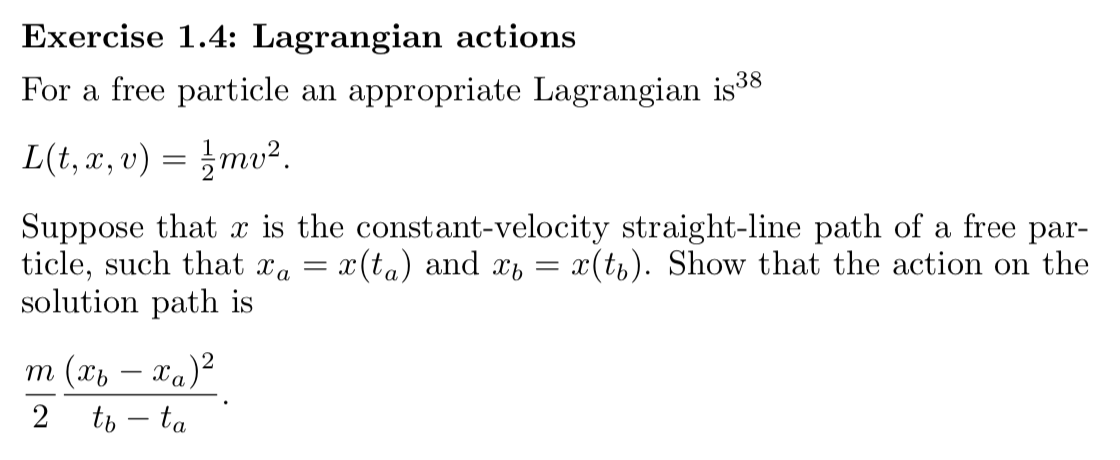
\includegraphics[width=400pt]{img/physics--classical-mechanics--sicm--1-4.png}
\end{mdframed}
The path function is
\begin{align*}
  x(t) = x_a + \frac{t - t_a}{t_b - t_a}(x_b - x_a).
\end{align*}
Therefore the velocity function is the constant function
\begin{align*}
  v(t) = (D x)(t) = \frac{x_b - x_a}{t_b - t_a}.
\end{align*}
Therefore the action is
\begin{align*}
  S[x](t_a, t_b) &= \int_{t_a}^{t_b}  \frac{1}{2}m \frac{(x_b - x_a)^2}{(t_b - t_a)^2} \d t \\
                 &= \frac{m}{2} \frac{(x_b - x_a)^2}{(t_b - t_a)^2}\int_{t_a}^{t_b} \d t \\
                 &= \frac{m}{2} \frac{(x_b - x_a)^2}{t_b - t_a}.
\end{align*}

% the dependence of the lagrangian on position is equal to the rate of change of the dependence of the
%  lagrangian on velocity.

\section{Haliakis: Optimisation and Optimal Control: Exercises}
\subsection{Sheet 1}
\subsubsection{1.1: Find extremising solutions of given functionals}
\begin{mdframed}
  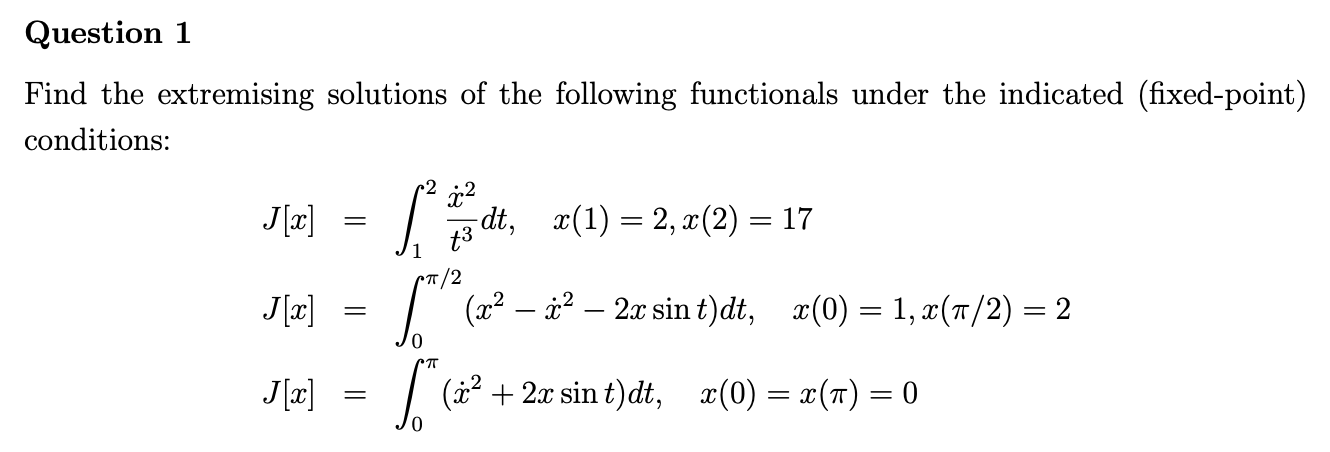
\includegraphics[width=400pt]{img/cov-haliakis-ooc-1-1.png}
\end{mdframed}
\begin{enumerate}
\item We have $f(t, x, \xdot) = \frac{\xdot^2}{t^3}$. So $\pdfdx = 0$ and $\pdfdxd = \frac{2\xdot}{t^3}$, and from
  the Euler-Lagrange equations we have that $x(t)$ satisfies
\begin{align*}
  \ddt \frac{2\xdot}{t^3} = 0.
\end{align*}
Therefore, letting $a, b, c$ be constants,
\begin{align*}
  \xdot &= at^3 \\
  x(t) &= bt^4 + c.
\end{align*}
From the endpoint conditions we have
\begin{align*}
  x(1) &= b + c = 2 \\
  x(2) &= 16b + c = 17 \\
  16b + 2 - b &= 17 \\
  b &= 1 \\
  c &= 1.
\end{align*}
So the extremising $x$ is $x(t) = t^4 + 1$. For this solution, the value of the functional is
\begin{align*}
  J[x]
  &= \int_1^2 \frac{(4t^3)^2}{t^3} \dt \\
  &= 16 \frac{t^4}{4}\Bigg|_1^2 \\
  &= 4 (16 - 1) = 60.
\end{align*}
Let's compare some other curves:
\begin{align*}
  x(t) &= bt^n + c \\
  x(1) &= 2 = b + c \implies c = 2 - b \\
  x(2) &= 17 = b2^n + 2 - b = b(2^n - 1) + 2 \implies b = 15/(2^n - 1)
\end{align*}

\begin{verbatim}
#+begin_src mathematica
n = 3.9; b = 15/(2^n - 1); x = b t^n + 2 - b; i = D[x, t]^2/t^3; Integrate[i, {t, 1, 2}]
#+end_src

#+RESULTS:
: 60.01726779228775
\end{verbatim}
So this appears to be correct \correct.

\item
  \begin{mdframed}
    Find the extremising solution to the functional
    \begin{align*}
      J[x] = \int_0^{\pi/2} x^2 - \xdot^2 - 2x\sin t \dt,
    \end{align*}
    subject to the endpoint conditions
    \begin{align*}
      x(0)   &= 1 \\
      x(\pi/2) &= 2.
    \end{align*}
  \end{mdframed}
  The integrand is $f(t, x, \xdot) = x^2 - \xdot^2 - 2x\sin t$, so $\pdfdx = 2x - 2\sin t$ and
  $\pdfdxd = -2\xdot$, and the Euler-Lagrange equations are
  \begin{align*}
    \dxdt (-2\xdot)  - \(2x - 2\sin t\) &= 0 \\
    \xddot + x &= \sin t.
  \end{align*}
  Let $V$ be a vector space of functions $\R \to \R$ and define $L:V \to V$ by $L(x) = \xddot + x$.

  To solve our differential equation, we first find the kernel of $L$. I.e. the set of functions $x$ that solve
  the homogeneous equation $\xddot + x = 0$.

  This is a Simple Harmonic oscillator: $x(t) = \sin t$ and $x(t) = \cos t$ are both solutions and so the
  kernel of $L$ is $\{A\sin t + B\cos t ~|~ A, B \in \R\}$.

  \todo{Should complex exponentials be used here?}

  Next we need a particular solution. We try (inspiration/online solutions) $x(t) = Ct\cos t$:
  \begin{align*}
    \xdot(t)/C      &= -t\sin t + \cos t \\
    \xddot(t)/C      &= -t\cos t - \sin t - \sin t \\
    \xddot(t) + x(t) &= -2C\sin t,
  \end{align*}
  so $x(t) = -\frac{1}{2}t\cos t$ is a particular solution, and the set of all solutions is
  $\{A\sin t + B\cos t - \frac{1}{2}t\cos t ~|~ A, B \in \R\}$.

  We now restrict this set to functions that satisfy the endpoint conditions:
  \begin{align*}
    A\sin 0 + B\cos 0 - \frac{1}{2}(0)\cos 0                     &= 1 \\
    B                                                            &= 1 \\
    A\sin (\pi/2) + B\cos (\pi/2) - \frac{1}{2}(\pi/2)\cos \pi/2 &= 2 \\
    A                                                            &= 2.
  \end{align*}
  So the function that is extremal for the given functional is
  \begin{align*}
    2\sin t + \cos t - \frac{t}{2}\cos t. ~~~~~~~ \correct
  \end{align*}
\item
  \begin{mdframed}
    Find the extremising solution to the functional
    \begin{align*}
      J[x] = \int_0^{\pi} \xdot^2 + 2x\sin t \dt,
    \end{align*}
    subject to the endpoint conditions
    \begin{align*}
      x(0) &= 1 \\
      x(\pi) &= 0.
    \end{align*}
  \end{mdframed}
  We have $f(t, x, \xdot) = \xdot^2 + 2x\sin t$ hence
  \begin{align*}
    \pdfdx  &= 2\sin t \\
    \pdfdxd &= 2\xdot,
  \end{align*}
  and the E-L equation is
  \begin{align*}
    \ddt \pdfdxd - \pdfdx &= 0 \\
    \xddot &= \sin t.
  \end{align*}
  The solution to which is $x(t) = -\sin t + C$. From $x(0) = 0$ we have $C = 0$, and
  this satisfies the other endpoint condition also.

  So the solution is $x(t) = -\sin t$. ~~~~~~~\correct

\end{enumerate}



\subsubsection{1.2: Lagrangian not explicitly dependent on t}

\begin{mdframed}
  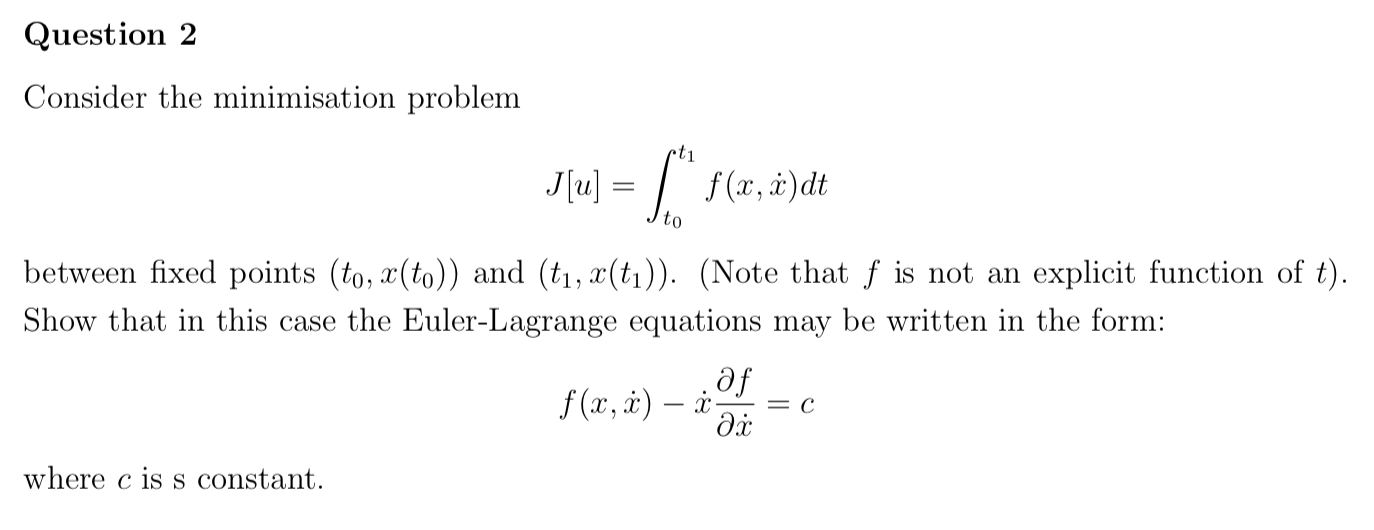
\includegraphics[width=400pt]{img/cov-haliakis-ooc-1-2.png}
\end{mdframed}
(Note that although $f$ does not depend \emph{explicitly} on $t$, it does depend on $t$ through its dependence on
$x(t)$ and $\xdot(t)$.)

Let $Q(t) = f(x, \xdot) - \xdot\pdfdxd$.

We are asked to show that the stated assumptions lead to the conclusion that
\begin{align*}
  \text{E-L condition holds} \iff Q(t) \text{ is constant}.
\end{align*}
First we examine the time derivative of $Q$:
\begin{align*}
  \ddt Q(t)
  &= \ddt \(f(x, \xdot) - \xdot \pdfdxd\) \\
  &= \xdot \pdfdx + \xddot \pdfdxd - \xdot \ddt \pdfdxd - \xddot \pdfdxd \\
  &= \xdot\(\pdfdx - \ddt \pdfdxd\).
\end{align*}
Note that this will be zero if $x$ is extremal.

So at this point we conclude that, if $x$ is an extremal function, then $Q(t)$ is constant.

Now, suppose $Q(t)$ is constant. Then its time derivative is zero. Therefore either $\xdot(t) = 0$ or the E-L
equations hold.

\begin{mdframed}
  \includegraphics[width=400pt]{img/zz.png}
\end{mdframed}

\subsubsection{1.3: Lagrangian not explicitly dependent on t}
\begin{mdframed}
  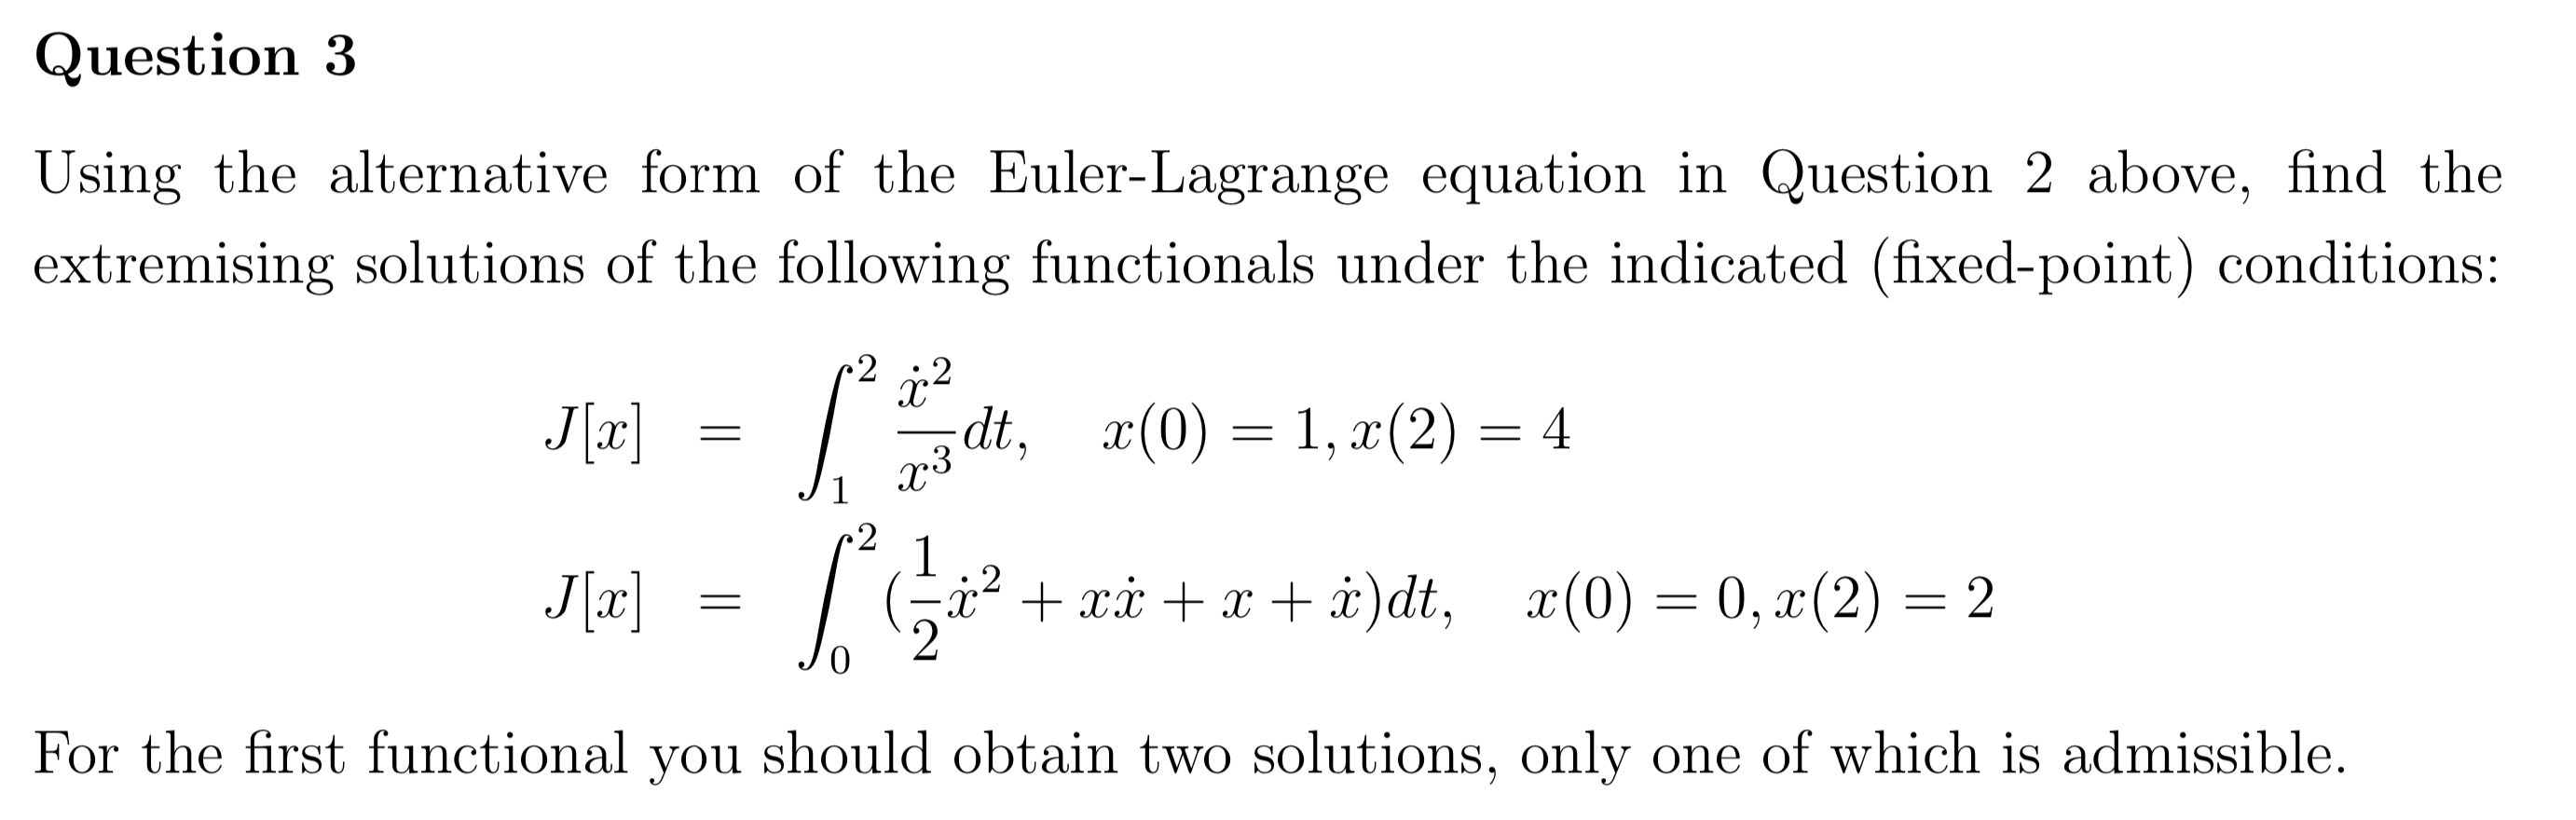
\includegraphics[width=400pt]{img/cov-haliakis-ooc-1-3.png}
\end{mdframed}

Recall that if the Lagrangian $f = f(x, \xdot)$ does not depend on $t$ {\it explicitly}, then $x$ is extremal iff it
satisfies the alternative form of the Euler-Lagrange equation
\begin{align*}
    f(x, \xdot) - \xdot\pdfdxd = \constant.
\end{align*}
\begin{enumerate}[label=(\alph*)]
\item We have $f(x, \xdot) = \frac{\xdot^2}{x^3}$. Therefore $\pdfdxd = \frac{2\xdot}{x^3}$, and the alternative form of E-L is
  \begin{align*}
    \frac{\xdot^2}{x^3} - \xdot \frac{2\xdot}{x^3} &= C_1 \\
    -\xdot^2       &= C_1x^3 \\
    x^{-3/2} \xdot &= C_2 \\
    \int x^{-3/2} \dx &= \int C_2 \dt \\
    -2x^{-1/2} &= C_2t + C_3 \\
    x &= \frac{1}{(C_3t + C_4)^2}.
  \end{align*}

  From the endpoint conditions, we have
  \begin{align*}
   x(0) = 1 &= \frac{1}{C_4^2} \\
   C_4      &= \pm 1 \\
   x(2) = 4 &= \frac{1}{(2C_3 + C_4)^2} \\
   (2C_3 + C_4)^2 &= \frac{1}{4}
\end{align*}
Therefore if $C_4 = 1$ then we have $C_3 = \frac{1}{2}\(\frac{1}{\pm\sqrt{2}} - \1\)$ and
\todo{incomplete}

\begin{minted}{wolfram}
x[t_] := 1 / (c3 t + c4)^2;
x[t] /. Solve[{x[0] == 1, x[2] == 4}, {c3, c4}]
\end{minted}

  #+RESULTS:
  \begin{align*}
    \left\{\frac{1}{\left(1-\frac{3 t}{4}\right)^2},\frac{1}{\left(1-\frac{t}{4}\right)^2},\frac{1}{\left(\frac{t}{4}-1\right)^2},\frac{1}{\left(\frac{3 t}{4}-1\right)^2}\right\}
  \end{align*}

\begin{mdframed}
  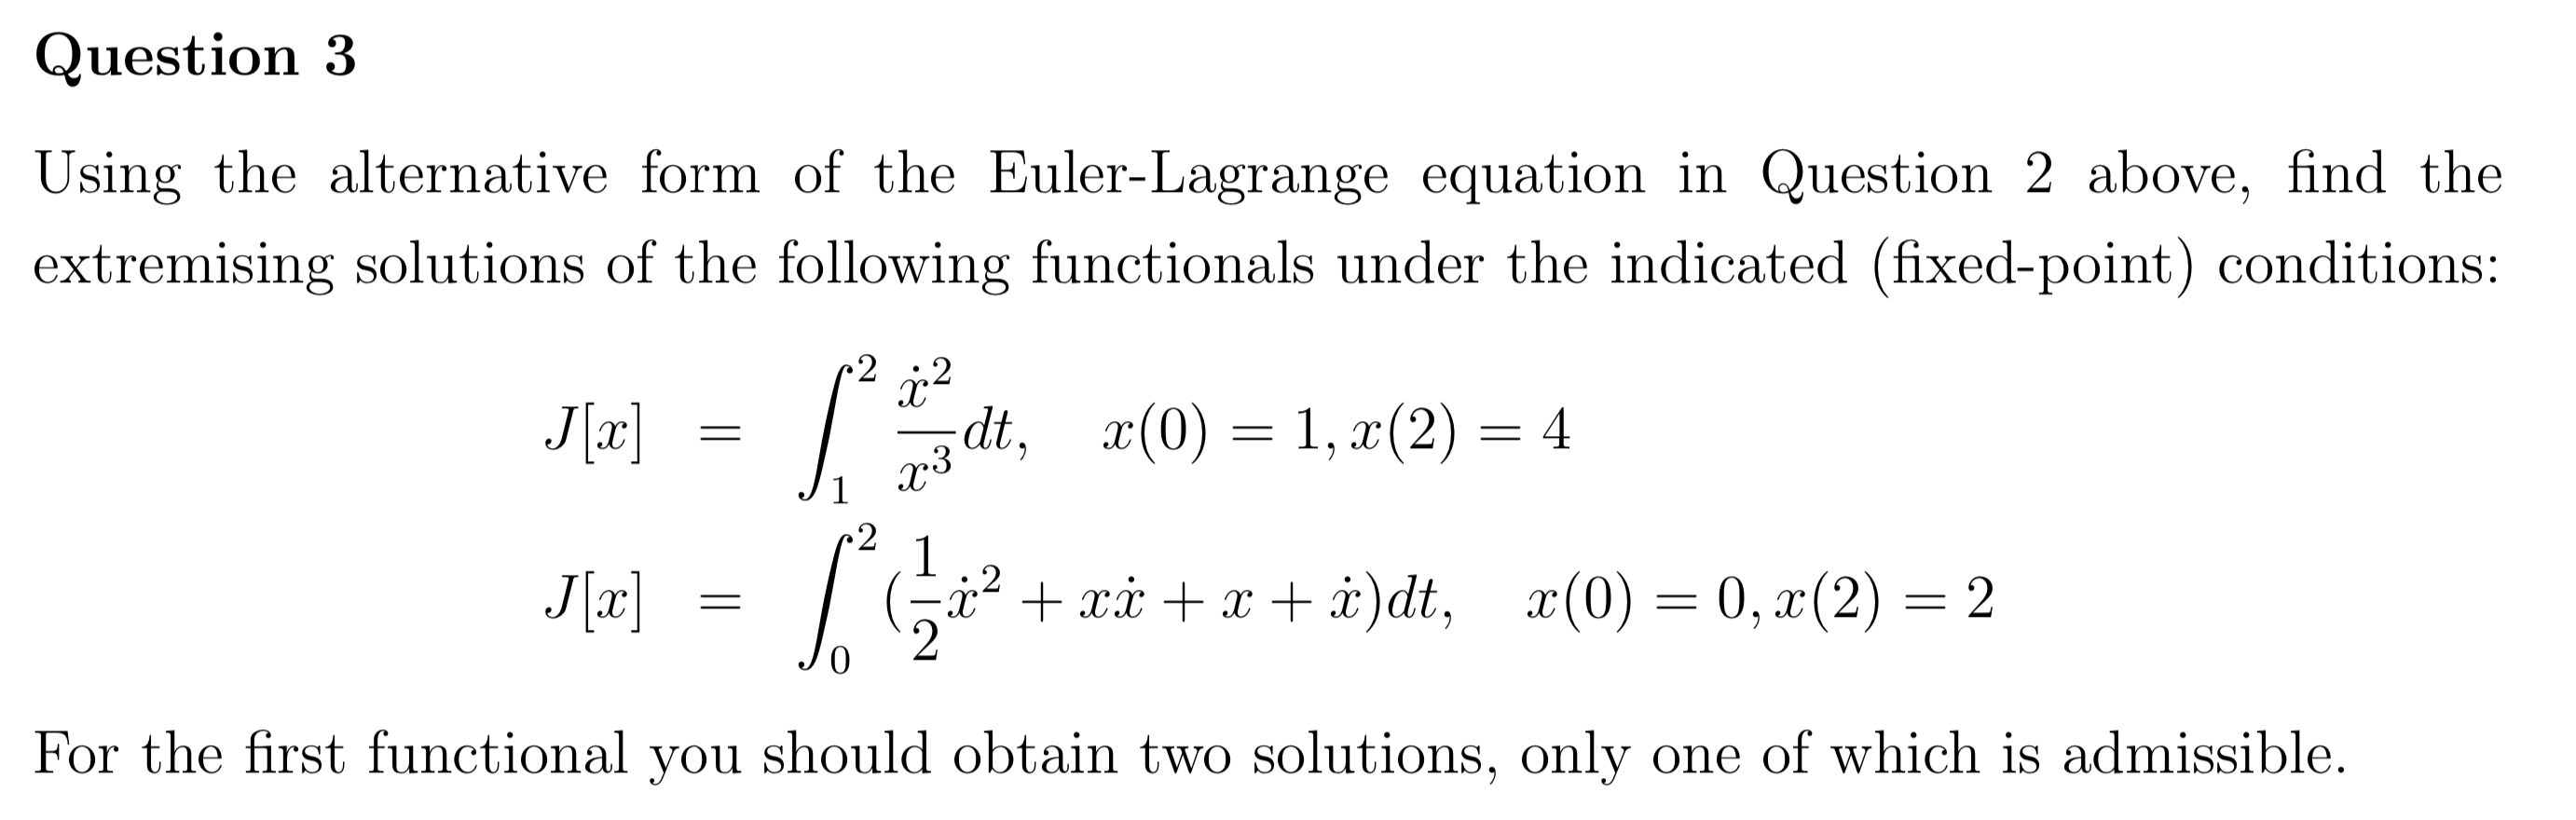
\includegraphics[width=400pt]{img/cov-haliakis-ooc-1-3.png}
\end{mdframed}

\item We have $f(x, \xdot) = \frac{1}{2}\xdot^2 + x\xdot + x + \xdot$ and so $\pdfdxd = \xdot + x + 1$ and the alternative form of E-L is
\begin{align*}
  f(x, \xdot) - \xdot\pdfdxd &= C_1 \\
  \frac{1}{2}\xdot^2 + x\xdot + x + \xdot - \xdot(\xdot + x + 1) &= C_1
\end{align*}



\end{enumerate}
\subsubsection{1.8: Find curve enclosing maximal area (Lagrange multiplier)}
\begin{mdframed}
  Among all curves of length $l$ in the upper-half $(x, y)$ plane passing through the points $(-a, 0)$
  and $(a, 0)$, find the one which together with the interval $[-a, a]$ encloses the largest possible area.
\end{mdframed}

To use Euler-Lagrange, we write this as a functional in the standard form. The integrand, which in general
is $f(x, y, y')$, here is simply $y(x)$.
\begin{align*}
  A[y] = \int_{-a}^{a} f(x, y, y') \dx = \int_{-a}^{a} y(x) \dx.
\end{align*}
Clearly there is no extremizing $y$ as things stand -- it could go as high as it likes as long as it comes back
to $(a, o)$ -- we need a constraint on the shape of $y$.

But let's see what happens if we try to use Euler-Lagrange at this stage anyway. We have $\pdfdy = 1$
and $\pdfdyp = 0$, and the Euler-Lagrange equations are
\begin{align*}
  \ddx \pdfdyp - \pdfdy = 0 - 1 = 0,
\end{align*}
so it looks like some assumption has been violated.

In any case, we have a constraint:
\begin{align*}
  \int_{-a}^a \sqrt{\dx^2 + \dy^2} &= l \\
  \int_{-a}^a \sqrt{1 + y'^2} \dx &= l \\
  \int_{-a}^a g(x, y, y') \dx &= l,
\end{align*}
where $g(x,y,y') = \sqrt{1 + y'^2}$.

So we use a Lagrange multiplier approach: we will maximize the functional
\begin{align*}
  A[y]
  &= \int_{-a}^{a} h(x, y, y') \dx \\
  &= \int_{-a}^{a} f(x, y, y') - \lambda g(x, y, y') \dx \\
  &= \int_{-a}^{a} y - \lambda \sqrt{1 + y'^2} \dx.
\end{align*}
We have $\pdhdy = 1$ and $\pdhdyp = \frac{-\lambda y'}{\sqrt{1 + y'^2}}$ and so the Euler-Lagrange equations are
\begin{align*}
  \ddx \pdhdyp - \pdhdy &= 0 \\
  \lambda \ddx \frac{y'}{\sqrt{1 + y'^2}} + 1 &= 0.
\end{align*}
Integrating, we have
\begin{align*}
  x + \lambda \frac{y'}{\sqrt{1 + y'^2}} &= C_1.
\end{align*}
Switch notation:

We have
\begin{align*}
  t + \lambda \frac{\xdot}{\sqrt{1 + \xdot^2}} &= C_1,
\end{align*}
therefore
\begin{align*}
  \lambda^2 \frac{\xdot^2}{1 + \xdot^2} &= (t - C_1)^2 \\
  \lambda^2 \xdot^2 &= (t - C_1)^2(1 + \xdot^2) \\
  \xdot^2(\lambda^2 - (t - C_1)^2) &= (t - C_1)^2 \\
  \xdot^2 &= \frac{(t - C_1)^2}{\lambda^2 - (t - C_1)^2} \\
  \xdot &= \frac{t - C_1}{\sqrt{\lambda^2 - (t - C_1)^2}} \\
        &= \ddt \sqrt{\lambda^2 - (t - C_1)^2}.
\end{align*}
Therefore on integrating again, we have
\begin{align*}
  (t - C_1)^2 + (x - C_2)^2 = \lambda^2.
\end{align*}

  The following attempts to approach the problem without Lagrange Multipliers didn't seem to get anywhere:

  Note that the curves in question need not be functions $y(x)$, so we will express the curves
  parametrically. In order to restrict ourselves to curves of length $l$ we will restate the problem
  as follows:

  Let $u \in (0, l)$ be a parameter measuring distance along the curve, and let $\chi$ be a suitable family of
  curves. We seek a curve $\r(u) = \vecMM{x(u)}{y(u)} \in \chi$ maximising the functional
\begin{align*}
  A[\r] = \int_0^l f(l, \r, \r') \d l,
\end{align*}
where $f(l, \r, \r')$ gives the rate of change of area with respect to $l$.

such that $\r(0) = \vecMM{0}{0}$ and $\r(l) = \vecMM{a}{0}$.

We want to find a curve that maximizes
\begin{align*}
  \int_0^l \d A.
\end{align*}
We can write this as
\begin{align*}
  \int_0^l A'(l) \d l
\end{align*}
where $A(l)$ is the area up to $l$.

We need to express $A'(l)$ in terms of...?

%%% Local Variables:
%%% TeX-master: "mathematics"
%%% TeX-command-extra-options: "-shell-escape"
%%% End:
